
\فصل{مفاهیم اولیه}


همواره مرسوم‌ترین راه برای بیانِ فیزیکِ کوانتوم، دنبال کردنِ سیرِ تاریخیِ رخدادها بوده، اما امروزه با به وجود آمدنِ رایانشِ کوانتومی، بسیاری از منابع از اصلِ موضوع‌های رایانش و اطلاعاتِ کوانتومی برای ورود به فیزیکِ کوانتوم استفاده می‌کنند و معتقدند این درگاه، باعث کم‌تر گمراه شدنِ افراد در گزاره‌های ناسازگار با شهودِ ما از طبیعت دارد.
\مرجع{aaronson2013}

\قسمت{حالت‌های کلاسیک و کوانتومی}
مفاهیمِ «حالت» و «گزار» در بخش‌های مختلفی از دانش استفاده شده و کاربردهای گوناگونی دارد، یکی از این کاربردها، در زنجیره‌های مارکوفی‌ست.

\زیرقسمت{زنجیرهٔ مارکوفی}
این بخش تنها مقدمه و مروری بر زنجیره‌های مارکوفی‌ست.

\شروع{نمایش}
برای نمایشِ بردارها از حروفِ کوچک و توپر 
\( \mathbf{a} \)
استفاده می‌کنیم و برای نمایشِ ماتریس‌ها از حروفِ بزرگِ تو‌پر
\( \mathbf{A} \)
نشان می‌دهیم.

برای نمایشِ ترانهاده بردارها و ماتریس‌ها از علامتِ
\( .^\intercal \)
استفاده می‌کنیم.

برای نشان دادنِ درایه‌ها نیز از زیروند به شکلِ
\( \mathbf{A}_{ij} \)
استفاده می‌کنیم.

همچنین بردارِ 
\( \mathbf{j} \)
نشان‌دهندهٔ بردارهایی با همهٔ عناصر یک است و
\( \mathbf{e_i} \)
برداری‌ست که تنها مؤلفهٔ \( i \)ام آن یک است و باقی صفر هستند.

برای بردارهای  مختلط از علامتِ 
\( .^* \)
برای مزدوج‌مختلطِ تک‌تکِ درایه‌های بردارها و ماتریس‌ها استفاده می‌کنیم.

همچنین
\begin{equation} .^\dagger = .^{*\intercal} \end{equation}
\پایان{نمایش}
یک زنجیرهٔ مارکوفی یک دنباله از متغیرهای تصادفی \( X_t \)‌ بر روی مجموعهٔ گسستهٔ حالت‌ها به نامِ 
\( \mathbf{S} \)
 است. با این شرط که توزیعِ متغیرِ تصادفیِ متغیر 
\( X_{t+1} \)
 امِ دنباله تنها بستگی به جملهٔ 
\( X_{t} \)
 ام دارد و احتمالاتِ شرطیِ این بستگی در طولِ این زنجیره ثابت هستند و می‌توان آن‌ها را با ماتریسِ گزار نشان داد به این ترتیب که برای همهٔ \( t \)ها
\begin{equation} (\mathbf{T})_{ij} = \Pr(X_{t+1} = j | X_t = i) \end{equation}

که اگر در کنارِ این ماتریس، بردارِ احتمال را تعریف کنیم
\begin{equation} (\mathbf{p}^t)_i = \Pr(X_t = j) \end{equation}
آن‌گاه می‌توان این خاصیت‌ها را در حالتِ کلی اثبات کرد.

\begin{equation} \mathbf{j}^\intercal \mathbf{p}^t = 1 \end{equation}

\begin{equation} \mathbf{T} \mathbf{j} = \mathbf{j} \end{equation}
\begin{equation} \mathbf{j}^\intercal \mathbf{T} = \mathbf{j}^\intercal \label{eq:markov-sum-invar} \end{equation}

و همچنین به شکلِ کلی می‌توان تحول را به این شکل بیان کرد.

\begin{equation} \mathbf{p}^t = \mathbf{T}^t \mathbf{p}^0 \end{equation}

می‌توان معادلهٔ 
\ref{eq:markov-sum-invar}
 را به شکلِ شفاهی این طور بیان کرد که جمعِ مؤلفه‌ها در گزارِ سیستم ناورداست. البته این طبیعی‌ست زیرا برای ما مطلوب است که بردارِ 
 \( \mathbf{p}^t \)
 همواره توزیعِ احتمال باقی بماند.

با توجه به این‌که این ماتریس گزار مثبت است خواص متعددی را می‌توان برای آن اثبات کرد، از جمله این‌که ویژه‌برداری با ویژه‌مقدارِ بیشینه (برابرِ یک) وجود دارد که حالتِ تعادلِ این سیستم پس از بی‌نهایت‌بار گزار است.
\مرجع{grinstead}

\زیرزیرقسمت{تضارب حالت‌ها}

دو زنجیرهٔ مارکوفی را در نظر بگیرید که (لااقل در ابتدا) مستقلاً کار می‌کنند. زنجیرهٔ اول در حالتِ 
\( \mathbf{p}^1 \)
و زنجیرهٔ دوم را در حالتِ 
\( \mathbf{p}^2 \) 
در نظر بگیرید. اگر بخواهیم مجموعِ دو زنجیره را با یک زنجیرهٔ بزرگ‌تر بیان کنیم

\begin{equation} \mathbf{p}^{\text{کل}} = \mathbf{p}^1 \otimes \mathbf{p}^2 \end{equation}

که در آن \(\otimes\) ضرب تانسوری‌ست.
و به همین شکل

\begin{equation} \mathbf{T}^{\text{کل}} = \mathbf{T}^1 \otimes \mathbf{T}^2 \end{equation}

حالا اگر بعد از تحولی به شکلِ مجزا یا به شکلِ هم‌بسته، از بردارِ حالتِ دو سیستم، به بردارِ حالتِ یکی از سیستم‌ها برسیم کافی‌ست

\begin{equation} \mathbf{p}^1_i = \sum_{j}^{\dim(\text{زنجیرهٔ دوم})} \mathbf{p}^{\text{کل}\intercal} \mathbf{e}^1_i \otimes \mathbf{e}^2_j \end{equation}

\زیرزیرقسمت{کمیت‌های مشاهده‌پذیر}

برای سیستمی که در حالتِ 
\(\mathbf{p}\)
قرار دارد، دسترسی به خودِ این بردار در عمل مقدور نیست و آن‌چه مشاهده می‌شود، کمیتِ مشاهده‌پذیری نظیرِ 
\( X \)
است که می‌توان آن را تابعی از حالت‌های سیستم درنظر گرفت، یعنی
\begin{equation} M : \{ 1 \dots n \} \to \mathbb{R} \end{equation}
که البته این تابع را می‌توان به شکلِ برداری نشان داد که در آن صورت، بیانِ کمیتی مثلِ امیدِ ریاضیِ آن ساده‌تر می‌شود

\begin{equation} \mathbb{E}[M] = \mathbf{M}^\intercal \mathbf{p} \end{equation}

\زیرقسمت{گزارهای کوانتومی}
سیستمِ احتمالاتی‌ای را (با \( n \) حالتِ مجزا) بگیرید که برای نمایشِ آن از برداری \( n \)-بعدی، مختلط و با اندازهٔ یک  به نامِ 
\(\mathbf{v}\)
بهره می‌گیریم به طوری‌که

\begin{equation} \Pr(i) = |\mathbf{v}_i|^2\end{equation}

به هر فضای برداری‌ای که یک ضربِ داخلی برروی آن تعریف شده، نظیرِ فضای برداریِ تعریف‌شده، «فضای هیلبرت» می‌گوییم.

\شروع{نمایش}
برای بردارهای مختلط، به جای 
\(\mathbf{v}\)
از
\(\ket{v}\)
استفاده می‌کنیم و همچنین برای
\(\mathbf{v}^\dagger\)
از 
\(\bra{v}\)
استفاده می‌کنیم.

همچنین
\(\braket{v}{u}\)
ضربِ داخلیِ دوبردار و 
\(\ket{v}\ket{u}\)
نمایشِ ساده‌ای از
\(\ket{v}\otimes\ket{u}\)
است.

و به ازای هر 
\(i \in \{ 0, \dots , n \}\)
\(\ket{i}\)
برداری‌ست که مؤلفهٔ \(i\)ام آن یک است.

در نهایت
\(\dyad{v}{u}\)
همان ماتریسِ
\(\mathbf{v}\mathbf{u}^\dagger\)
است.

ماتریس‌ها با علامتِ توپر نشان داده نمی‌شوند و همچنین \(I\) ماتریس همانی‌ست.

\پایان{نمایش}

در ادامه نشان خواهیم‌داد این گونه‌حالت‌ها چیزی فراتر از زنجیرهٔ مارکوفی هستند.
برای گزارِ این سیستم، باید از ماتریس‌های حافظِ اندازه (ماتریس‌های یکانی) استفاده کنیم، به این ترتیب هر 
\(U \in SU(n)\)
\زیرنویس{
\(SU(n)\)
گروه ماتریس‌های یکانیِ 
\(n\times n\)
هستند.}
یک گزار برای این سیستم است.

\شروع{مثال}[تبدیل هادامارد]
\برچسب{مثال:هادامارد}
فرض کنید سیستمی با دو حالتِ مجزا داریم و آن را یک کیوبیت می‌نامیم.
اگر بگیریم

\begin{equation} \ket{0} := \begin{pmatrix} 1 \\ 0 \end{pmatrix} \end{equation}
\begin{equation} \ket{1} := \begin{pmatrix} 0 \\ 1 \end{pmatrix} \end{equation}

همچنین اگر بگیریم

\begin{equation} \ket{+} := \frac{1}{\sqrt{2}} (\ket{0} + \ket{1}) \end{equation}
\begin{equation} \ket{-} := \frac{1}{\sqrt{2}} (\ket{0} - \ket{1}) \end{equation}

این‌دو بردار هردو توزیعِ احتمالاتی به شکلِ 
\(\mathbf{p} = \begin{pmatrix} 1/2 \\ 1/2 \end{pmatrix} \)
دارند.

و اگر این تحول را در نظر بگیریم

\begin{equation} H = \frac{1}{2} \begin{pmatrix} 1 & 1 \\ 1 & -1 \end{pmatrix} \end{equation}

آن‌گاه تحتِ این تحول، دو بردارِ مثبت و منفی که توزیعِ احتمالِ یک‌شکل داشتند به دو بردار با توزیع‌های متفاوت می‌روند که این‌چنین رفتاری با زنجیرهٔ مارکوفی قابلِ‌توصیف نیست.

این مثال نشان می‌دهد که این تئوری اندکی با تئوریِ احتمالِ مرسوم متفاوت است.
\پایان{مثال}

نکتهٔ دیگری که موردِ‌ توجه است این است که برخلافِ \(T\)، گزارِ \(U\) حتماً وارون‌پذیر است که این نکته‌ای‌ست که در بخش‌های دیگر بیشتر موردِ توجه قرار می‌گیرد.

\زیرزیرقسمت{اندازه‌گیری}

یکی از بخش‌های مبهمِ مکانیکِ کوانتومی، اندازه‌گیری‌ست. تصور کنید که سیستمی کوانتومی در حالتِ
\(\ket{v}\)
قرار دارد. اگر یک مشاهده یا اندازه‌گیریِ فیزیکی انجام بگیرد، بردارِ حالتِ سیستم با احتمالِ
\(\Pr(i) = |\braket{e_i}{v}|^2\)
به بردارِ 
\(\ket{e_i}\)
تبدیل می‌شود. به این عمل «فروریزش» می‌گویند.

\شروع{مثال}
مانندِ مثالِ قبل، یک کیوبیت را تصور کنید 

\شروع{شمارش}[-]
\فقره سیستم در حالتِ اولیهٔ 
\(\ket{+}\)
باشد.

\فقره تحول \(H\) را روی آن اعمال شود.

\فقره اندازه‌گیری را انجام شود.
\پایان{شمارش}

نتیجهٔ این فرایند به این شکل است که با احتمالِ
\(\Pr(0) = 1\)
حالتِ \(0\) مشاهده می‌شود.

حالا سناریوی دیگری را درنظر بگیرید که در ابتدا یک اندازه‌گیری نیز انجام می‌گیرد.

\شروع{شمارش}[-]
\فقره سیستم در حالتِ اولیهٔ 
\(\ket{+}\)
باشد.

\فقره یک اندازه‌گیریِ اولیه انجام می‌شود.

\فقره تحول \(H\) را روی آن اعمال شود.

\فقره اندازه‌گیری را انجام شود.
\پایان{شمارش}

می‌توان محاسبه کرد که حاصلِ این فرایند با احتمالِ
\(\Pr(0) = \frac{1}{2}\)
حالتِ \(0\) و با احتمالِ
\(\Pr(1) = \frac{1}{2}\)
حالتِ \(1\) مشاهده می‌شود.

این آزمایش تأثیرِ مفهومِ رمبش را نشان می‌دهد. به این ترتیب که می‌توان آزمایشِ مشابهی برای زنجیره‌های مارکوفی تعریف کرد و خواهیم دید که اندازه‌گیری هیچ‌تأثیری در زنجیره‌های مارکوفی ندارد.

\پایان{مثال}

به طورِ مشابه، برای آن‌چه در خصوصِ کمیت‌های مشاهده‌پذیر در زنجیرهٔ مارکوفی گفتیم، دسترسی به بردارِ حالتِ یک سیستم 
\(\ket{v}\)
و حتی توزیع احتمالاتِ آن مقدور نیست.

در ساده‌ترین حالت در نظر بگیرید که کمیتِ مشاهده‌پذیری به نامِ \(M\) داریم که به هر حالتِ سیستم (یا به عبارتی دیگر هر بردار از پایهٔ متعامد‌یکهٔ فضا) مانندِ 
\(\ket{i}\)
یک عدد 
\(\lambda_i \in \mathbb{R}\)
نسبت می‌دهد.

می‌دانیم که آن‌گاه

\begin{equation} \mathbb{E}[M] = \sum_i \lambda_i \Pr(i) = \sum_i \lambda_i |\braket{i}{v}|^2 = \sum_i \lambda_i \braket{v}{i}\braket{i}{v} 
\label{eq:expval-quantum} \end{equation}

که حالا اگر ماتریسِ زیر را تعریف کنیم
\begin{equation} \hat{M} := \sum_i \lambda_i \dyad{i} \end{equation}

آن‌گاه، می‌توان معادلهٔ 
\ref{eq:expval-quantum}
را به شکلِ زیر نوشت
\begin{equation} \mathbb{E}[M] = \ev{\hat{M}}{v} \end{equation}

اما حقیقتِ ماجرا این است که در یک سیستمِ فیزیکی، ممکن است چند پایهٔ متعامدیکه برای  حالت‌های مربوط به مشخصه‌های مختلف وجود داشته‌باشد.

\شروع{مثال}[آزمایشِ اشترن-گرلاخ]

\برچسب{مثال:اشترن-گرلاخ}

با اغماض می‌توان الکترون‌ها را آهن‌رباهای کوچکی در نظر گرفت که سه مؤلفه دارند و این سه مؤلفه جهت آهن‌ربا را مشخص می‌کند. به این کمیتِ برداری، «اسپین» می‌گوییم.
\علامت‌زیرنویس

پس مؤلفه‌های اسپین را می‌توان در هرکدام از راستاهای \(x\) و \(y\) و \(z\) اندازه‌گیری کرد. در نتیجه باید بتوان سه عملگر به شکل 
\(\hat{X}\)
و 
\(\hat{Y}\)
و 
\(\hat{Z}\)
تعریف کرد.

در آزمایش اشترن-گرلاخ با اندازه‌گیری پیاپی این عملگرها نتایجی دور از انتظار می‌بینیم، برای مثال اگر با اندازه‌گیری‌های پیاپی 
\(\hat{Y}\)
ببینیم که سیستم در راستای \(y\) اسپینی برابر 
\(\frac{1}{2}\)
\علامت‌زیرنویس
دارد، اگر حال اندازه‌گیری 
\(\hat{X}\)
را ترتیب بدهیم، اطلاعاتی که از اسپین در راستای \(y\) به دست آورده‌ایم نیز دیگر معتبر نیست.

در نتیجهٔ این آزمایش، ساده‌ترین مدلی که این رفتار را توصیف کند به شرحِ زیر است که این سیستم علی‌رغمِ این‌که سه مؤلفه برای اندازه‌گیری دارد، حالتِ آن برداری نظیر 
\(\ket{\psi}\)
در فضای دوبعدی‌ست و عملگرهای گفته‌شده برابر با ماتریس‌هایی به شکلِ زیر است.

\begin{equation} \hat{X} = \frac{1}{2} \begin{pmatrix} 0 & 1 \\ 1 & 0 \end{pmatrix} \end{equation}
\begin{equation} \hat{Y} = \frac{1}{2} \begin{pmatrix} 0 & -i \\ i & 0 \end{pmatrix} \end{equation}
\begin{equation} \hat{Z} = \frac{1}{2} \begin{pmatrix} 1 & 0 \\ 0 & -1 \end{pmatrix} \end{equation}

\پایان{مثال}
\متن‌زیرنویس{این تعریف به هیچ‌وجه تعریف دقیقی از اسپین به عنوانِ یک کمیت ذاتی در ذرات صحیح نیست و تنها مثال ملموسی‌ست برای استفاده از آن در سیاقِ رایانشِ کوانتومی}
\متن‌زیرنویس{مقدارِ دقیق‌ترِ آن 
\(\frac{\hbar}{2}\)
است که برای سادگی، مقدارِ 
\(\hbar\)
را که یک ثابتِ جهانی به نامِ ثابتِ کاهیدهٔ پلانک است، یک فرض می‌کنیم.}

یک مثالِ معروف‌تر از این، «مکان» و «تکانه» هستند که هردو پایه‌های متعامد‌یکه‌ای برای فضای حالت‌های یک ذره هستند. در نتیجهٔ این، نمی‌توان مکان و تکانه را همزمان اندازه‌گیری کرد و همچنین با اندازه‌گیریِ آن‌ها به ترتیب می‌توان به اصلِ عدمِ قطعیت 
\زیرنویس{اصلِ عدمِ قطعیت، اصلی‌ست که بیان می‌کند هرگونه اندازه‌گیری‌ای که مکان و تکانه را به ترتیب با خطای
\(\Delta x\)
و
\(\Delta p\)
اندازه‌گیری کند، این نامساوی برقرار است
\begin{equation} \Delta x \Delta p \ge \frac{\hbar}{2} \end{equation}
}
را اثبات کرد.

\زیرزیرقسمت{مدلِ کوانتوم-احتمالاتی}

حالا می‌توان مدلی را تصور کرد که سیستم، به شکلِ احتمالاتی، در حالاتِ کوانتومیِ متعدد باشد. یعنی دنباله‌ای از حالت‌ها داریم 
\(\ket{v_1}\dots \ket{v_n} \)
داریم که سیستم با احتمالاتِ نظیرِ
\( p_1 \dots p_n \)
در این حالات حضور داشته‌باشد.

سیستم‌های این‌چنینی را می‌توان با ترکیبِ مدلِ احتمالاتی و کوانتومی بررسی کرد، اما برای بررسیِ ساده‌تر، می‌توان کمیتِ زیر را تعریف کرد که ماتریسِ چگالی نام دارد و نمایندهٔ این توزیعِ احتمالاتی از توزیع‌هاست.

\begin{equation} \rho := \sum_{i=1}^n p_i \dyad{v_i} \end{equation}

حالا اثرِ یک تحولِ کوانتومی که یک ماتریسِ یکانی مانند \(U\) است، برروی این ماتریسِ چگالی، به شکلِ زیر است.

\begin{equation} \rho \mapsto U \rho U^\dagger \end{equation}

و همچنین، با اندازه‌گیریِ یک کمیت، مانندِ 
\(M\)
امیدِ ریاضیِ آن از رابطهٔ زیر به دست می‌آید.

\begin{equation}  \mathbb{E}[M] = \Tr(\rho \hat M)\end{equation}

بررسیِ تحولاتِ این سیستم‌ها، با مفهومی به نامِ کانال انجام می‌گیرد که خارج از این مقال است.

\زیرزیرقسمت{تضاربِ حالت‌ها}

اگر دو سیستمِ کوانتومیِ مجزا با حالت‌های 
\(\ket{v}\)
و
\(\ket{u}\)
 داشته‌باشیم، آن‌گاه حالتِ کلیِ سیستم
\( \ket{v}\otimes\ket{u} \)
خواهدبود.

در این صورت اگر عملگری مانند \(U\) را فقط برروی سیستمِ اول اثر بدهیم، آنگاه اثرِ آن بر کلِ سیستم به شکلِ
\(U \otimes I\)
خواهد بود. به شکلی مشابه می‌توان عملگری را فقط روی سیستمِ دوم اثر داد یا عملگری را روی هردو سیستم به شکلِ همزمان اثر داد که در نتیجهٔ آن، بردارِ حاصل، به شکلِ ضربی مثلِ 
\( \ket{v'}\otimes\ket{u'} \)
قابلِ بیان نباشد.

در کلی‌ترین حالت، برداری که متعلق به دو فضا باشد را بتوان به شکلِ زیر نوشت

\begin{equation} \ket \psi = \sum_i \ket{a_i}\otimes\ket{b_i} \end{equation}

حالا فرض کنید فضای دوم را در پایه‌ای دلخواه اندازه‌گیری می‌کنیم. و نتیجهٔ آن بردارِ \(\ket{b_i}\) در سیستمِ اآنگاه سیستم با احتمالِ
\(|\braket{b_i}{\psi}|^2\)
در حالتِ
\(\frac{\braket{b_i}{\psi}}{|\braket{b_i}{\psi}|}\)
قرار می‌گیرد.
ذکرِ این نکته لازم است که حاصلِ 
\(\braket{b_i}{\psi}\)
یک بردار در فضای اول است و نه یک عدد.

این‌طور می‌توان گفت که پس از اندازه‌گیریِ فضای دوم، یک حالتِ احتمالاتیِ کوانتومی داریم که با آن را با یک ماتریسِ چگالی نشان می‌دهیم.

\begin{equation} 
    \rho_{\text{فضای اول}} = \sum_i |\braket{b_i}{\psi}|^2 \frac{\braket{b_i}{\psi}}{|\braket{b_i}{\psi}|} \frac{\braket{\psi}{b_i}}{|\braket{b_i}{\psi}|} = \sum_i \braket{b_i}{\psi}\braket{\psi}{b_i} = \Tr_{\text{فضای دوم}} \dyad{\psi} 
\end{equation}

که با ساده‌سازی به ردِ جزئی می‌رسیم.


\زیرقسمت{تفاوت‌های سیستم‌های کوانتومی و کلاسیک}
همچنان که در مثالِ \رجوع{مثال:هادامارد} گفته‌شد، سیستم‌های کوانتومی قابلیت‌هایی متعددی مزیدِ بر سیستم‌های کلاسیک دارند. آن‌چه در آن مثال دیده‌شد به نوعی قابلیتِ پنهان کردنِ اطلاعاتی در سیستم بود که خود را در یک اندازه‌گیریِ ساده نشان نمی‌دهد.

در ادامه در قالبِ یک مثال، به بررسیِ هم‌بستگی‌های کوانتومی می‌پردازیم که «درهم‌تنیدگی» نامیده می‌شود.

\شروع{مثال}[آزمایشِ بل]

یک بازی را تصور کنید، که داور به هرکدام از دو بازیکن (آلیس و باب) یک بیت ارسال می‌کند. درنظر بگیرید 
\(x\)
را به آلیس و 
\(y\)
را به باب ارسال می‌کند.

آلیس و باب نمی‌توانند با هم هیچ پیامی ردوبدل کنند. حالا، آلیس و باب، هرکدام برحسبِ استراتژیِ خود یک بیت را به داور برمی‌گردانند. تصور کنید دو بیت را 
\(a\)
و
\(b\)
باشند.
آلیس و باب هردو با هم پیروز می‌شوند اگر و تنها اگر 
\begin{equation}
    a \XOR b = x \AND y
\end{equation} 

حالا یک‌بار در نظر می‌گیریم که استراتژیِ هرکدام، به شکلِ تعینی باشد، یعنی

\begin{equation}
\begin{cases}
    a_x = f(x) \\
    b_y = g(y) 
\end{cases}
\end{equation}
اگر فرض بگیریم که هریک از مقادیرِ 
\(x\) و \(y\) 
هم‌احتمال باشند، آنگاه برای احتمالِ پیروزی، برای هر استراتژی‌ای خواهیم داشت

\begin{equation}
    \label{معادله:بل-بازی}
    \Pr(\text{پیروزی}) \le \frac{3}{4}
\end{equation}

حالا اگر استراتژیِ هرکدام از آلیس و باب، به شکلِ احتمالاتی و وابسته به یک متغیرِ تصادفیِ مشترک مانندِ 
\(\lambda\)
باشد

\begin{equation}
\begin{cases}
    \Pr(a | x, \lambda) = f(a, x, \lambda) \\
    \Pr(b | y, \lambda) = g(b, y, \lambda)
\end{cases}
\end{equation}
در این صورت، باز هم همان حد برای احتمالِ پیروزی برقرار است.

اما اگر به‌جای متغیرِ تصادفیِ مشترک، یک حالتِ کوانتومی بینِ آلیس و باب به اشتراک گذاشته شود، به طوری‌که سیستمِ کوانتومیِ مسئله، از دو زیرسیستمِ دوحالته تشکیل شده‌است که زیرسیستمِ اول در اختیارِ آلیس و زیرسیستمِ دوم در اختیارِ باب است. (که در زیر فوق با اندیس‌ها مشخص شده‌اند)

\begin{equation}
    \ket\psi = \frac{1}{\sqrt{2}} (\ket{0}_A\ket{0}_B + \ket{1}_A\ket{1}_B) 
\end{equation}

حالا اگر برای تعیینِ استراتژی هرکدام از بازیکنان از اندازه‌گیری استفاده کنند، یعنی با توجه به ورودی
(\(x\) و \(y\))
یک پایهٔ متعامد برای اندازه‌گیری انتخاب کند \علامت‌زیرنویس و از نتیجهٔ آزمایش، خروجیِ خود را انتخاب کند، یعنی اگر
\( \{\ket{A^0_0}, \ket{A^0_1} \} \)
و 
\( \{\ket{A^1_0}, \ket{A^1_1} \} \)
دو پایهٔ متعامدِ برای اندازه‌گیری در زیرسیستمِ آلیس باشند و به شکلِ مشابهی برای باب، بردارهای 
\(B\)
را داشته‌باشیم، می‌توانیم به این شکل بنویسیم که
\begin{equation}
    Pr(a, b | x, y) = \abs{\bra\psi \ket{A^x_a} \ket{B^y_b}}^2
\end{equation}

دلیلِ این‌که نمی‌توان این احتمال را برای آلیس و باب به شکلِ مجزا نوشت این است که هرکدام از این‌دو، نخست اندازه‌گیری را انجام دهند، برروی استیتِ کلیِ سیستم تأثیر می‌گذارند، هرچند که این تأثیر، همچنان نمی‌توان هیچ پیامی را منتقل کرد، اما شکلِ خاصی از هم‌بستگی را به وجود می‌آورد که در سیستم‌های کلاسیک دیده نمی‌شوند و درنتیجه باعث می‌شود که احتمالِ پیروزی می‌تواند به 
\( \frac{1 + 2\sqrt{2}}{2} \simeq 0.85 \)
برسد که این نقضِ نامساویِ \رجوع{معادله:بل-بازی} است.
\مرجع[ناموضعیت در مکانیکِ کوانتومی]{karimipour}
\پایان{مثال}
\متن‌زیرنویس{اندازه‌گیری در پایهٔ متعامدِ دلخواه، هم‌ارزِ انجامِ یک تحولِ یکانیِ مناسب و سپس اندازه‌گیری در پایهٔ اصلی است. پس اگر تحول‌های یکانی همگی در دسترس باشند، اندازه‌گیری در هر پایه‌ای ممکن است. دربارهٔ در دسترس بودنِ تحول‌ها در \رجوع{زیرزیرقسمت:مدارهای-کوانتومی} بررسی می‌شود.}

\قسمت{رایانشِ کوانتومی و کلاسیک}

\زیرقسمت{مدل رایانش}

\شروع{نمایش}
یک الفبا مانند 
\(\Sigma\)
، یک مجموعه از علامت‌هاست.
اگر 
\(s \in \Sigma\)
یکی از آن علامت‌ها باشد
\(s s\)
یا
\(s^2\)
یک کلمهٔ ساخته‌شده با تکرارِ آن علامت است و همچنین 
\(\Sigma^2\)
 مجموعهٔ کلمه‌ها با طول دو است. (و به همین‌ترتیب برای طول‌های بیشتر)

از عملگرِ 
\(.^*\)
برای بیانِ مجموعه‌های کلمه‌های آن الفبا (با طول صفر یا بیشتر) استفاده می‌کنیم. همچنین برای هر 
\(s \in \Sigma^*\)
عملگرِ \(|.|\) طولِ آن را بیان می‌کند.

برای یک 
\(s \in \Sigma^*\)
اگر 
\(\Sigma = \mathbb{Z}_N\)
یعنی اعداد کوچک‌تر از \(N\) باشد، آن‌گاه عددی که این بازنمایی را در مبنای \(N\) دارد با
\(\overline{s}\)
نمایش می‌دهیم.
\پایان{نمایش}

مدل‌های مختلفی برای بیانِ رایانش کوانتومی وجود دارد اما پر استفاده‌ترینِ آن‌ها مدلِ مداری‌ست که به سادگی قابلِ ساخت از روی مدلِ کلاسیکِ مداری‌ست.

در مدل‌های محاسباتی، یک مسئله را به شکلی استاندارد که قابل محاسبه باشد بیان می‌کنیم. برای سادگی، در این بخش فرض می‌کنیم که مسئله‌ای که قصد حلِ آن را داریم، تابعی به شکلِ
\(f: \mathbb{Z}_2^* \to \mathbb{Z}_2\)
است.

\زیرزیرقسمت{خانوادهٔ مدارهای یکنواخت و غیرِیک‌نواخت}
 
یک مدار \(C\)، یک گرافِ جهت‌دارِ غیرِ مدور است که سه دسته گره برروی آن مشخص می‌کنیم.

\شروع{شمارش}[-]
\فقره گره‌های ورودی: گره‌هایی با درجهٔ ورودیِ صفر هستند که هرکدام نمایانگر یکی از ورودی‌های مسئله است
هستند.

\فقره گره‌های گیت: گره‌هایی با درجهٔ ورودی و خروجی‌شان ناصفر هستند که هرکدام نمایانگر یک گیت از مجموعهٔ گیت‌های مجاز در مدار است که تعدادِ ورودی‌ها و تعدادِ خروجی‌های مشخصی دارد. برای ما این مجموعه شاملِ 
\(\AND\)
و 
\(\OR\)
هرکدام با دو ورودی و 
\(\NOT\)
 با یک ورودی است.

\فقره گره‌های خروجی: گره‌هایی با درجهٔ خروجی صفر که نمایندهٔ خروجیِ مسئله هستند (با توجه به تعریف تابع به شکلِ گفته شده، تنها یک گره خروجی داریم)

\پایان{شمارش}

برروی این مدار، توابعِ زیر را تعریف می‌کنیم
\شروع{شمارش}[-]
\فقره
\(\size(C)\):
تعدادِ گره‌های گیت در مدار

\فقره
\(\depth(C)\):
طولِ طولانی‌ترین مسیر در مدار
\پایان{شمارش}
با توجه به تعریفی که از مدار ارائه شد، اندازهٔ ورودی‌های آن ثابت است و برای حلِ مسئله به شکلی که گفته شد، نیاز به یک خانواده از مدارها داریم. خانوادهٔ مدار \(F\)، یک دنباله از مدارها به شکلِ
\((F_1, F_2, \dots)\)
است که \(F_i\) برای ورودی با طولِ \(i\) تابعِ \(f\) را محاسبه می‌کند.


اگر تابعِ \(f\) با یک خانوادهٔ مدار \(F\) قابلِ محاسبه باشد، به طوری که برای
\(\size(F_i)\)
(به عنوانِ تابعی از \(i\)) داشته‌باشیم
\(\size(F_i) \in \mathcal{O}(poly(i))\)
آن‌گاه می‌گوییم مسئلهٔ محاسبهٔ \(f\) عضو کلاس 
\(\mathbf{P}/poly\)
است.

مثالِ ساده‌ای وجود دارد که نشان می‌دهد این مدل از ماشین تورینگ قوی‌تر است.
\شروع{مثال}[این مثال صرفاً به خاطرِ علاقهٔ شخصیِ نویسنده این‌جاست و بار علمی‌ای ندارد.]
فرض کنید مسئلهٔ \(h\) به شکلِ 
\( h: \mathbb{Z}_2^* \to \mathbb{Z}_2\)
برای ماشینِ تورینگ غیرقابل محاسبه است. (می‌دانیم چنین مسئله‌ای وجود دارد)

می‌دانیم که به ازای هر 
\(s \in \mathbb{Z}_2^\star\)
می‌توان عددی طبیعی به آن نسبت داد که به این شکل ساخته‌می‌شود
\(n_s = \overline{1 s}\)
به سادگی می‌توان گفت این تبدیل یک‌به‌یک و پوشاست.

حال ابتدا مسئلهٔ دیگری به شکلِ 
\(f: 1^\star \to \mathbb{Z}_2 \)
می‌سازیم که در آن 
\begin{equation} f(1^{n_s}) = h(s) \end{equation}
آنگاه طبیعتاً برای هرطولی از ورودیِ \(f\) یک مدار وجود دارد که خروجیِ لازم را تولید کند. (اما تولیدِ خودِ مدار کارِ سختی‌ست و این مهم همان‌چیزی‌ست که به آن توجه نشده‌بود)

پس خانوادهٔ مدار از ماشین تورینگ قوی‌تر عمل می‌کنند. 
\پایان{مثال}

با توجه به مثالِ گفته‌شده، خانوادهٔ مدارهای یکنواخت را تعریف می‌کنیم که در آن هرکدام از
\(F_i\)
ها به سادگی (در زمان چندجمله‌ای) توسط یک مدل محاسباتی قابل توصیف باشند.

حالا اگر مسئله‌ای با یک خانوادهٔ مدار یکنواخت \(F\) قابلِ محاسبه باشد، اگر
\(\size(F_i) \in \O{poly(i)}\)
آن‌گاه می‌گوییم مسئلهٔ محاسبهٔ \(f\) عضو کلاس 
\(\mathbf{P}\)
است.
 
پس از آن، مسئله‌ای مانندِ \(g\) را تصور کنید که برای ورودی، علاوه‌بر \(x\)، یک رشته به نامِ \(w\) می‌گیرد به طوری که 
\(
    |w| \in \O{poly(|x|)}
\)
طولِ این رشته نسبت به طولِ \(x\) به شکلِ چندجمله‌ای باشد.


این ورودیِ \(w\) را به شکلِ نوعی سرِ نخ برای \(f(x)=1\) استفاده می‌کنیم، یعنی فرض کنید

\begin{equation}
    \begin{cases}
    \exists w ~ g(x \cdot w) = 1 \Leftrightarrow f(x) = 1 \\
    \forall w ~ g(x \cdot w) = 0 \Leftrightarrow f(x) = 0 \\
    \end{cases}
\end{equation} 
اکنون اگر مسئلهٔ \(g\) که مسئلهٔ \(f\) به همراهِ سرنخ است (و از مسئلهٔ \(f\) آسان‌تر است) عضوِ کلاسِ 
\( \mathbf{P} \)
باشد می‌گوییم که مسئلهٔ \(f\) خود عضوِ کلاسِ
\( \mathbf{NP} \)
است.

برای تعریفِ چند کلاسِ دیگر، تصور کنید یک مدار به شکلِ احتمالاتی کار می‌کند یا برای سازگاری با تعریف‌های قبل، این‌بار بگیرید مسئلهٔ \(g\) علاوه بر ورودیِ \(x\)، یک رشته از اعدادِ تصادفی به طولِ چندجمله‌ای را می‌گیرد که آن را \(r\) می‌نامیم. اگر \(g\) خود عضوِ 
\( \mathbf{P} \) 
باشد و داشته‌باشیم

\begin{equation}
    \Pr(g(x \cdot r) = f(x)) \ge \frac{2}{3}
\end{equation} 
آن‌گاه \(f\) عضوِ کلاسِ 
\( \mathbf{BPP} \)
است. 
\مرجع{arora}
\زیرنویس{
کلاس‌های
\( \mathbf{P} \)
،
\( \mathbf{NP} \)
و
\( \mathbf{BPP} \)
هیچ‌گاه به این شکل تعریف نمی‌شوند. شکلِ اولیهٔ تعریفِ آن‌ها مبتنی بر ماشینِ تورینگ است و بعد در طیِ قضیه‌هایی، اثبات می‌شود که به این شکل قابلِ نوشتن هستند.
}
 
 
\زیرزیرقسمت{مدارهای کوانتومی}
\برچسب{زیرزیرقسمت:مدارهای-کوانتومی}
حالا تصور کنید یه سیستمِ \(d\)-حالتهٔ 
کوانتومی داریم. به این سیستم «کیودیت» می‌گوییم. در حالتی که 
\(d=2\)
به این سیستم «کیوبیت» می‌گوییم.

اگر یک سیستم متشکل از \(n\) کیوبیت در نظر بگیریم، چنان‌چه پیشتر گفته‌شد، می‌توان تحول‌هایی را به شکلِ محلی برروی یکی یا چندتا از این کیوبیت‌ها (به عنوانِ یک زیرسیستم از سیستمی بزرگ‌تر) اعمال کرد.

از این رو می‌توان متصور شد که اگر گیت‌های پایهٔ کوانتومی را تعریف کنیم، بتوان مدارِ کوانتومی را تعریف کرد که به شکلِ مشابهی، شاملِ گره‌های زیر خواهد بود \مرجع{deutsch}

\شروع{شمارش}[-]
\فقره گره‌های ورودی: مشابهِ حالتِ قبل اما به شکلِ حالتِ کوانتومی است. (البته می‌دانیم که هر حالتِ کلاسیکی لزوماً یک حالتِ کوانتومی نیز هست)
\فقره گره‌های خروجی: مشابهِ حالتِ قبل اما به شکلِ حالتِ کوانتومی است.
\فقره گره‌های گیت‌های کوانتومی: مشابهِ حالتِ قبل اما ذکرِ این نکته لازم است که گیت‌های پایه در مدارهای کوانتومی، نمی‌توانند شاملِ
\(\AND\)
و
\(\OR\)
باشند چرا که این گیت‌ها باید فضای مبدأ و مقصد یکسانی داشته‌باشند (درجهٔ ورودی و خروجی‌شان یکی باشد) و تحولِ متناظر با آن‌ها وارون‌پذیر باشد. در اصل هر گیت باید یک ماتریس یکانی باشد.
\فقره گرهِ اندازه‌گیری: یک اندازه‌گیری در پایهٔ 
\( \ket{0} \)
و 
\( \ket{1} \)
انجام می‌شود که طبیعتاً درجهٔ ورودیِ آن یک و درجهٔ خروجیِ آن نیز یک است.
\پایان{شمارش}


یکی از مشهورترین مجموعهٔ گیت‌های پایه مجموعهٔ گیتِ \(H\) از مثالِ \رجوع{مثال:اشترن-گرلاخ} و همچنین \(T\) و \(\CNOT\)
است که به شکلِ زیر تعریف می‌شوند. \مرجع{boykin}

\begin{equation}
    T := \begin{pmatrix}
        1 & 0 \\
        1 & e^{i\frac{\pi}{4}} \\
    \end{pmatrix}
\end{equation}

\begin{equation}
    \CNOT := \dyad{0} \otimes I + \dyad{1} \otimes \NOT 
\end{equation} 

که در این بین، \(T\) و \(H\) عملگرهای تک‌کیوبیتی هستند اما  \(\CNOT\) یک عملگرِ دوکیوبیتی است.

حالا به شکلِ مشابهی همان توابع برروی مدارهای کوانتومی نیز تعریف می‌شوند و همچنین تعریفِ خانوادهٔ مدار و یکنواختی نیز به همین ترتیب تعمیم داده‌می‌شود.
 
\زیرزیرقسمت{کلاس‌های محاسباتی کوانتومی}

به شکلِ مشابهی، برای مسئله‌ای به شکلِ 
\( f: \{ 0, 1\}^* \to \{ 0, 1\}\)
داریم 
\زیرنویس{می‌دانیم که مدارهای کوانتومی، فضای مبدا و مقصدِ یکسانی دارند، از این رو، پیاده‌سازیِ تابعی به شکلِ فوق، می‌تواند به این شکل انجام بگیرد که ورودی به شکلِ کوانتومی داده می‌شود و پس از انجامِ یک عملیاتِ یکانی، برروی یک کیوبیتِ خاص، اندازه‌گیری رخ می‌دهد و حاصلِ اندازه‌گیری به عنوانِ خروجیِ سیستم لحاظ می‌شود.}
که اگر با خانوادهٔ یکنواختی از مدارهای کوانتومی، به نامِ
\( Q \)
قابل محاسبه باشند، به طوری‌که 
\( \size(Q_i) \in \O{poly(i)} \) 
آن‌گاه می‌گوییم که این مسئله عضوِ کلاسِ
\( \mathbf{EQP} \)
\زیرنویس{
\lr{exact quantum polynomial}}
است.

در ادامه، اگر بگیریم که مدارِ کوانتومی، همواره درست عمل نکند اما با احتمالِ خوبی پاسخِ درست بدهد، یعنی به شکلِ فرمال داشته‌باشیم
\begin{equation}
    \Pr(f(x) = Q_i(x)) \ge \frac{2}{3} 
\end{equation} 
آنگاه می‌گوییم که مسئله در کلاسِ
\( \mathbf{BQP} \)
قرار دارد.

در این‌جا بدونِ اثبات، چند گزاره درخصوصِ کلاس‌های محاسباتیِ گفته‌شده را بررسی می‌کنیم.
\مرجع{watrous}
\مرجع{aaronson2010}

\begin{eqnarray}
    \mathbf{P} \subseteq \mathbf{EQP} \subseteq \mathbf{BQP} \\ 
    \mathbf{P} \subseteq \mathbf{BPP} \subseteq \mathbf{BQP} \\
    \mathbf{NP} \not\subset \mathbf{BQP} \\
    \mathbf{NP} \not\supset \mathbf{BQP}
\end{eqnarray}
\زیرقسمت{الگوریتم‌های پایه‌ای در رایانش کوانتومی}

برای بررسیِ الگوریتم‌های کوانتومی، نیاز به شیوه‌ای برای ییانِ آن‌ها داریم، هرچند تلاش‌های بسیاری برای طراحیِ زبان‌ها و حساب‌ها برای رایانشِ کوانتومی صورت گرفته، اما برای حفظِ یک‌پارچگی با شیوهٔ بیانِ الگوریتم‌های کوانتومی، از شیوه‌های نموداری، نظیرِ شکلِ مدارِ کوانتومی و حسابِ 
\lr{ZX}
استفاده نمی‌کنیم.
\مرجع{deutsch}
\مرجع{backens}
\مرجع{selinger}
ذکرِ این نکته هم لازم است که روش‌های شکلی تعمیم‌پذیر نیستند. از طرفی زبان‌های کوانتومی اغلب ساختارِ مشترکی در خصوصِ ساختارداده‌ها و عملیات‌های کوانتومی دارند اما از نظرِ عملیات‌های کلاسیک، تفاوت‌های بسیاری دارند. از این‌رو برای تشریحِ الگوریتم‌های کوانتومی از شبه‌کد کمک خواهیم گرفت. هرچند ساختارِ این شبه‌کد کاملاً گویاست اما برای حفظِ صحت و دقت، در پیوست آن را از نظرِ نحوی و معنایی بررسی می‌کنیم.

% TODO add appendix 

ذکرِ این نکته لازم است که الگوریتم‌های کوانتومیِ گسترده‌ای برای کاربردهای متنوعی وجود دارند
\مرجع{lokhov}
\مرجع{montanaro}
\مرجع{jordan}
 اما در این مقال، تمرکز برروی الگوریتم‌های پایه‌ای خواهندبود که به زعمِ نویسنده می‌توانند کاربردی در مسائلِ هندسهٔ محاسباتی داشته‌باشند.


\زیرزیرقسمت{الگوریتمِ دویچ-جوزا}

اگر جعبه‌سیاهی داشته‌باشیم که مدارِ تابعِ 
\( o : \mathbb{Z}_2^n \to \mathbb{Z}_2 \)
باشد و برای این تابع داشته‌باشیم که حتماً یکی از حالت‌های زیر برقرار است

\شروع{شمارش}[-]
\فقره تابع ثابت است.
\فقره تابع متوازن است به این معنی که به ازای نیمی از ورودی‌ها 
\( o(x) = 1 \)
و برای نیمی دیگر
\( o(x) = 0 \)
\پایان{شمارش}
حالا مسئله این است که تشخیص بدهیم تابعِ \(o\) در کدام‌یک از دسته‌های فوق می‌افتد.

با استفاده از هر مدلِ  کلاسیکی، نظیرِ خانوادهٔ مدارها، قابلِ تصور است که برای جوابِ قطعی، نیاز به حداقل
\(2^{n-1}+1\)
بار استفاده از جعبه‌سیاهِ مذکور داریم.

اما به شکلِ کوانتومی، اگر فرض کنیم که همین مدارِ تابعِ \(o\) را داریم و برای این‌که این مدار، خواصِ یک مدارِ کوانتومی (وارون‌پذیری و یکی‌بودنِ فضای مبدأ و مقصد) را داشته‌باشیم، تحولِ یکانیِ \(O\) را به شکلِ زیر تعریف کنیم

\begin{equation}
    O = \sum_{x \in \mathbb{Z}_2^n, y \in \mathbb{Z}_2} \dyad{x, y \XOR o(x)}{x, y}
\end{equation} 

این تعمیم برروی \(n+1\) کیوبیت تعریف شده‌است که \(n\) کیوبیتِ اول، نقشِ ورودیِ \(o\) را دارند و کیوبیتِ آخر، محلِ ذخیرهٔ خروجیِ \(o\) است.

حالا شبهِ‌کدی مانندِ \رجوع{الگوریتم:دویچ-جوزا} را درنظر بگیرید.

\شروع{الگور}[آ]
\begin{latin}
\begin{lstlisting}
H : 1 qubit gate = 1/2 * [1,  1;
                          1, -1]
function IsConstant(O: n+1 qubit gate)   
    // Qubits:
    x : n qubit state
    y : 1 qubit state

    // Algorithm:
    // stage 1, initialization
    for i : integer from 1 to n
        Initiate x[i] to |0>
    Initiate y to |1>

    // stage 2, parallization
    for i : integer from 1 to n
        Apply H on x[i]
       
    Apply H on y
        
    // stage 3, query
    Apply O on x, y
    
    // stage 4, interfere (fourier transform)
    for i : integer from 1 to n
        Apply H on x[i]

    // stage 5, measurement
    is_constant : boolean = true
    for i from 1 to n
        result : boolean = Measure on x[i]
        if (result)
            is_constant = false
            
    return is_constant
\end{lstlisting}
\end{latin}
\شرح{دویچ-جوزا}
\برچسب{الگوریتم:دویچ-جوزا}
\پایان{الگور}

برای تحلیلِ دقیقِ این الگوریتم، حالتِ کیوبیت‌ها را در پایانِ هر مرحله بررسی می‌کنیم

\begin{equation}
    \ket{\psi_1} = \ket{0^n}_x \ket{1}_y
\end{equation}
سپس با انجام شدنِ عملگرِ \(H\) برروی تک‌تکِ گیت‌ها، خواهیم داشت
\begin{equation}
    \ket{\psi_2} = \frac{1}{\sqrt{2^{n+1}}}\sum_{i = 0}^{2^n - 1} \ket{i}_x (\ket{0}_y - \ket{1}_y)
\end{equation}
\begin{align}
    \ket{\psi_3} &= \frac{1}{\sqrt{2^{n+1}}}\sum_{i = 0}^{2^n - 1} \ket{i}_x (\ket{o(i)}_y - \ket{\NOT o(i)}_y) \\
     &= \frac{1}{\sqrt{2^{n+1}}}\sum_{i = 0}^{2^n - 1}(\ket{0}_y - \ket{1}_y)
\end{align}
حالا با اعمالِ دوبارهٔ \(H\)ها برروی \(x\)ها، می‌دانیم که حالتِ \(y\) تغییری نخواهد کرد.
\begin{equation}
    \ket{\psi_4} = (H^{\otimes n}_x \frac{1}{\sqrt{2^{n+1}}}\sum_{i = 0}^{2^n - 1}  (-1)^{o(i)}\ket{i}_x ) \otimes (\ket{0}_y - \ket{1}_y)
\end{equation}
با اضافه کردنِ این نکته که درصورتی پاسخ 
\lr{\lstinline{is_constant}}
برابر با درست است که تمامِ بیت‌های خروجیِ \(x\) برابر با صفر باشند، یعنی
\begin{align}
    \Pr(\text{\lr{\lstinline{is_constant}}}) &= \norm{\bra{0^n}_x \ket{\psi_4}}^2 \\
     &= \abs{\bra{0^n}H^{\otimes n}_x \frac{1}{\sqrt{2^{n}}}\sum_{i = 0}^{2^n - 1}  (-1)^{o(i)}\ket{i}_x}^2 \\
     &= \frac{1}{2^n}\abs{(\frac{1}{\sqrt{2^{n}}}\sum_{i = 0}^{2^n - 1} \bra{i}) (\sum_{i = 0}^{2^n - 1}  (-1)^{o(i)}\ket{i})}^2 \\
     &= \frac{1}{2^{2n}}\abs{\sum_{i = 0}^{2^n - 1} (-1)^{o(i)}}^2
\end{align}
تنها نکتهٔ ریاضیاتیِ استفاده‌شده در این اثبات این است که عملگرهای \(H\) می‌توانند از نظرِ ریاضی برروی بردارِ ترانهاده/مزدوج 
\( \bra{0^n} \)
که در سمتِ راستشان قرار گرفته‌است اثر کنند.

در نتیجه می‌بینیم که برای حالتی که \(o\) مقدارِ ثابتی دارد، این احتمال برابر با یک و برای حالتِ متوازن این احتمال دقیقاً برابر با صفر است.

پس این الگوریتم که تنها یک‌بار از جعبه‌سیاهِ مذکور استفاده می‌کند، می‌تواند به شکلِ قطعی به مسئله پاسخ بدهد.
\مرجع{deutsch-joza}

برای تشریحِ بیشترِ آن‌چه که باعثِ این افزایشِ سرعت شد، می‌توان به این نکته اشاره کرد که همزمانیِ بررسیِ همهٔ حالت‌ها، در کنارِ ابزاری که عملکردی مشابهِ تبدیلِ فوریه دارد (تبدیلِ هادامارد) که در فضای کوانتومی به سرعت پیاده‌سازی می‌شود، امکانِ این نتیجه‌گیریِ سریع را فراهم آورده‌است. اما به طورِ کلی، در این الگوریتم و الگوریتم‌های بعدی، آن‌چه عمومیت دارد، ساختاری شبیه به سیستمِ احتمالاتی‌ست با این تفاوت که احتمالاتِ منفی‌ای دارد که با هم می‌توانند تداخلِ سازنده یا مخرب داشته‌باشند.

\زیرزیرقسمت{الگوریتم زیرگروهِ آبلیِ پنهان و کاربردهای آن}
می‌دانیم که گروهِ محدود، به یک مجموعهٔ محدود، مانندِ \(G\) و یک تابع که آن را ضربِ گروه می‌نامیم و به شکلِ 
\(\cdot: G \times G \to G\)
تعریف می‌شود می‌گوییم که خواصِ زیر را دارا باشد
\شروع{شمارش}[-]
\فقره شرکت‌پذیری: برای هر \(a, b, c \in G\) داشته‌باشیم 
\((a \cdot b) \cdot c = a \cdot (b \cdot c)\)
\فقره عنصرِ همانی: وجود داشته‌باشد \(I \in G\) که برای هر \(g \in G\) داشته‌باشیم
\(g \cdot I = I \cdot g = 1\)
\فقره عنصرِ وارون: برای هر عنصری نظیرِ \(g \in G\) داشته‌باشیم 
\(g^{-1} \in G\)
که  
\(g \cdot g^{-1} = g^{-1} \cdot g = I\)
\فقره جابه‌جایی (تنها در گروه‌های آبلی): برای هر \(a, b \in G\) داشته‌باشیم
\(a \cdot b = b \cdot a\) 
\پایان{شمارش}
همچنین زیرگروه، گروهی‌ست که زیرمجموعهٔ گروهی بزرگ‌تر با همان ضرب است و هم‌دستهٔ یک زیرگروه مانندِ \(H\) به مجموعه‌هایی می‌گویند که برای هر \(g \in G\) به شکلِ زیر تعریف می‌شوند
\begin{equation}
    gH = \{gh | h \in H\}
\end{equation}
و مولد‌های گروه، به کمینه عناصری می‌گویند که از بستارِ ضربِ آن‌ها در خود، همهٔ عناصرِ گروه به دست می‌آیند.

اگر گروهی محدود و آبلی به نامِ \(G\) داشته‌باشیم و تابعی به شکلِ
\(f : G \to S\)
نیز داده‌شده‌است که \(S\) یک مجموعهٔ دلخواه است.
اگر زیرگروهی به نامِ \(H\) وجود داشته‌باشد که برای \(f\) داشته‌باشیم که

\begin{equation}
    f(x) = f(y) \Leftrightarrow \text{\(x\) و \(y\) در یک هم‌دستهٔ زیرگروه \(H\) قرار دارند} \Leftrightarrow xH = yH
\end{equation}
آنگاه مسئله یافتنِ \(H\) (به معنای یافتنِ مولدهای آن گروه) است.

پیش از بررسیِ دقیقِ الگوریتم، به بررسیِ تعمیمِ تبدیلِ فوریه در فضای گروه‌های آبلیِ محدود می‌پردازیم. بدونِ اشاره به تئوریِ بازنماییِ گروه‌ها، مجموعهٔ توابعِ 
\(G \to \mathbb{C}\)
را در نظر بگیرید، این توابع تشکیلِ یک فضای برداری را می‌دهند، یک پایهٔ بدیهی برای این فضا، توابعِ زیر هستند

\begin{equation}
    \delta_g(x) = \begin{cases}
    1 & g=x \\
    0 & g \ne x
    \end{cases}
\end{equation}
بدونِ اثبات بپذیریم که یک پایهٔ نابدیهی برای این فضا، مجموعهٔ توابعی هستند که خواصِ زیر را دارند 
\مرجع{dandavati}
\begin{eqnarray}
    \abs{\chi_k(x)} = 1 \\
    \chi_k(I) = 1 \\
    \chi_k(x \cdot y) = \chi_k(x) \cdot \chi_k(y) 
\end{eqnarray}

که این اعدادِ \(k\) را نیز می‌توان با عناصرِ گروه جایگزین کرد اگر یک سریِ کمینهٔ مولد برای \(G\) درنظر بگیریم و آن را 
\(\mathrm{gen}(G)\)
بنامیم
\begin{eqnarray}
\chi_I(x) = 1 \\
\chi_g(g') = e^{\delta_{gg'}\frac{2i\pi}{\mathrm{order}(g)}} & \text{اگر \(g, g' \in \mathrm{gen}(G)\)} \\
\chi_{a \cdot b}(x) = \chi_a(x) \chi_b(x) 
\end{eqnarray}

لازم به ذکر است که مرتبهٔ \(g\) کوچک‌ترین عددی‌ست که \(g^{\mathrm{order}(g)} = 1\) یا به عبارتی دیگر
\begin{equation}
    \mathrm{order}(g) = |\{ g^z | z \in \mathbb{Z}\}|
\end{equation}

آن‌چه گفته‌شد، تعریفِ دو پایه برای مجموعهٔ توابعِ \(G \to \mathbb{C}\) بود که همین دو پایه برای فضای حالت‌های کوانتومیِ سیستمی که حالت‌های کلاسیکِ آن همان عناصرِ \(G\) است نیز برقرار است.

از این رو، می‌توان یک تحولِ یکانی در این فضا تعریف کرد که این تغییرِ پایه را صورت می‌دهد

\begin{equation}
    \mathrm{QFT} := \frac{1}{\sqrt{\abs{G}}} \sum_{a, b} \chi_a(b) \dyad{b}{a}  
\end{equation}

که این تعریف را تبدیلِ فوریهٔ کوانتومی می‌گیریم. لازم به ذکر است که به ازای گروهی خاص، (\(\mathbb{Z}_2\)) برابر با تبدیلِ هادامارد خواهد بود.

الگوریتمِ زیر را در نظر بگیرید

\شروع{الگور}[آ]

\begin{latin}
\begin{lstlisting}
function SampleFromHperp(G : Group, f: Hilbert(G × S) gate) {
    qft : Hilbert(G) gate = QFT of G, defined above
    
    x : Hilbert(G) state
    y : Hiblert(S) state
    
    // stage 1, initialization and applying oracle
    Initiate x to |I>
    Apply qft on x
    // or any other way to make x = sum |g>
    Initiate y to |0>
    
    Apply f on x, y
    
    // stage 2, collapsing into a constant set
    Measure on y
    
    // stage 3, applying QFT to extract generators
    Apply qft on x
    
    // stage 4, select a generator
    Measure on x
     
}
\end{lstlisting}
\end{latin}
\شرح{زیرگروهِ پنهان}
\برچسب{الگوریتم:زیرگروه-پنهان}
\پایان{الگور}

در مرحلهٔ اول، ابتدا تلاش می‌شود که حالتی به شکل
\(\frac{1}{\sqrt{\abs{G}}}\sum_{g \in G} \ket{g}_x\)
تولید شود که برحسبِ شکلِ ذخیره‌سازی و ساختارِ گروه، به شکل‌های متفاوتی می‌توان این کار را انجام داد، اما آن‌چه با همین ابزار قابلِ پیاده‌سازی‌ست، استفاده از تبدیلِ فوریه برروی عنصرِ همانی‌ست که این حالت را تولید می‌کند. سپس با اعمال \(f\) که تبدیل به عملیاتی یکانی شده، به حالتی به شکلِ زیر خواهیم رسید

\begin{equation}
    \ket{\psi_1} = \frac{1}{\sqrt{\abs{G}}}\sum_{g \in G} \ket{g}_x\ket{f(g)}_y
\end{equation}

سپس با اندازه‌گیری در فضای دوم، به برهم‌نهی از حالاتی می‌رسیم که مقدارِ 
\(f(g)\)
برای آن‌ها برابر بوده، یعنی یک هم‌دستهٔ \(H\)

\begin{equation}
    \ket{\psi_2} = \frac{1}{\sqrt{\abs{H}}} \sum_{h \in H} \ket{sh}_x \ket{f(s)}_y
\end{equation}

و پس از آن با اعمالِ تبدیلِ فوریهٔ مذکور، خواهیم داشت

\begin{equation}
    \ket{\psi_3} = \frac{1}{\sqrt{\abs{H} \abs{G}}} \sum_{h \in H} \sum_{g \in G} \chi_{s \cdot h}(g)\ket{g}_x \ket{f(s)}_y
\end{equation}

به سادگی می‌توان اثبات کرد که 
\begin{equation}
    \sum_{k = 0}^{\mathrm{order}(g) - 1} \chi_{g^k}(x) = \begin{cases} \mathrm{order}(g) & \chi_g(x) = 1 \\
0 & \chi_g(x) \ne 1 \end{cases}
\end{equation}
و همین تعمیم برای جمع برروی زیرگروه نیز وجود دارد که با استفاده از آن، می‌توان نوشت 

\begin{align}
    \ket{\psi_3} &= \frac{1}{\sqrt{\abs{H} \abs{G}}} \sum_{g \in G} \chi_s(g) \sum_{h \in H} \chi_{h}(g)\ket{g}_x \ket{f(s)}_y \\
    &= \frac{\sqrt{\abs{H}}}{\sqrt{\abs{G}}} \sum_{g \in H^\perp} \chi_s(g) \ket{g}_x \ket{f(s)}_y
\end{align}

که در رابطهٔ فوق \(H^\perp\) باید به شکلِ زیر تعریف شود
\begin{equation}
    H^\perp := \{g ~|~ \chi_h(g) = 1 ~ \forall h \in H\}
\end{equation}

نتیجهٔ اندازه‌گیریِ آخر، همان نمونه‌گیری از گروهِ \(H^\perp\) است و با دانستنِ این گروه، خودِ گروهِ \(H\) نیز دانسته می‌شود.\مرجع{kitaev}
\زیرنویس{شیوهٔ یافتنِ مولدهای \(H\) با استفاده از \(H^\perp\) در حالتِ کلی خارج از این مقال است}

در ادامه، در یک مثالِ کاربردی، به یافتنِ دورهٔ تناوبِ یک تابع می‌پردازیم که خود در تجزیهٔ اعداد استفاده می‌شود.
\زیرنویس{
ارتباطِ مثالِ مذکور با تجزیهٔ عددِ \(N\) نیز به این صورت است که با دانستنِ \(r\) اگر \(r\) زوج باشد، آن‌گاه معادلهٔ زیر می‌تواند منتج به تجزیهٔ عدد شود.
\begin{equation}
    (a^\frac{r}{2} + 1)(a^\frac{r}{2} - 1)\mod N = 0
\end{equation}
}

\شروع{مثال}[محاسبهٔ دورهٔ تناوب]
فرض کنید گروهِ اصلیِ مسئله
\(\mathbb{Z}_{Q}\)
(با عملِ جمع) باشد، آن‌گاه تابعِ \(f\) را به شکلِ زیر تعریف کنیم
\begin{equation}
 f(x) = a^x \mod N
\end{equation}
که طبیعتاً اعدادِ \(a\) و \(N\) دانسته‌شده هستند به طوری‌که 
\(\gcd(a, N) = 1\)

حالا زیرگروهی که این تابع برروی آن ثابت است
\(\{ 0, r, 2r, \dots Q - r \}\)
است اگر \(Q/r\) عددِ صحیحی باشد.

اگر الگوریتمِ مذکور برروی این مسئله اجرا شود، می‌دانیم که برای گروهِ گفته‌شده

\begin{equation}
    \chi_a(b) = e^{2i\pi\frac{ab}{Q}}
\end{equation}
که در نتیجهٔ آن، برای هر حاصلِ اندازه‌گیری مانندِ \(m\) خواهیم‌داشت
\begin{equation}
    \chi_r(m) = 1 \Rightarrow mr = kQ
\end{equation}
که در آن \(k\) عددی نامعلوم اما صحیح است و اگر چندبار \(m\) را اندازه بگیریم، مسئلهٔ به دست آوردنِ \(r\) به مسئلهٔ باقی‌ماندهٔ چینی تبدیل می‌شود و قابلِ حل است.

تنها نکتهٔ باقی‌مانده این ضمانت است که \(\frac{Q}{r}\) صحیح است که نشان داده‌شده حتی درصورتِ صحیح نبودنِ این نسبت، با قیدهایی، این الگوریتم با احتمالِ خوبی همچنان به‌درستی عمل می‌کند.
\مرجع{shor}
\پایان{مثال}

\زیرزیرقسمت{الگوریتم‌های جست‌وجو، شمارش و تقویت}
\برچسب{بخش:گروور}

یک تابع به شکلِ
$D \to \mathbb{Z}_2$
داده‌شده است که از مجموعهٔ محدودِ $D$ به اعدادِ صفر و یک می‌رود.
مسئله، پیدا کردنِ عنصر/عنصرهایی از $D$ هستند که به ازای آن‌ها
$f(s) = 1$.
این مقادیر را مجموعهٔ 
$T := \{ s | f(s) = 1\}$
 می‌نامیم و
این مسئله را جست‌وجوی نامرتب نیز می‌توان نامید.

حالا در فضای هیلبرتی که پایه‌هایش اعضای $D$ هستند می‌توانیم برداری به شکلِ زیر تعریف کنیم

\begin{equation}
    \ket{D} = \frac{1}{\sqrt{\abs{D}}} \sum_{e \in D} \ket{e}
\end{equation}
و همچنین یک عملگر و یک بردار به شکلِ زیر تعریف می‌کنیم
به این منظور اگر تعریف کنیم این یک عملگرِ خطی در فضای $x$ باشد
\begin{equation}
    \mathbb{P}_T := \sum_{x \in T} \dyad{x} 
\end{equation}
\begin{equation}
    \ket{T} :=  \frac{1}{\sqrt{\abs{T}}} \sum_{x \in T} \ket{x}
\end{equation}
که واضح است که 
$\mathbb{P_T} \ne \dyad{T}$.

اگر فرض بگیریم مداری (تنها متشکل از گیت‌های پایه و بدونِ اندازه‌گیری) به نامِ $G$ داریم که عملیاتِ زیر را انجام می‌دهد، و طبیعتاً می‌توان انتظار داشت که وارونِ این مدار را نیز داشته‌باشیم
\begin{equation}
    \ket{D} = G\ket{e_1}
\end{equation}
که $e_1$ یک عنصرِ دلخواه و مشخص از مجموعهٔ $D$ باشد،

فرض می‌کنیم که $f$ را نیز مشابهِ الگوریتم‌های قبل به شکلِ زیر داشته‌باشیم
\begin{equation}
    F = \sum_{x \in D, y \in \mathbb{Z}_2} \dyad{x, y \XOR f(x)}{x, y}
\end{equation}

همچنین عجیب نیست که به هرشکلی که برای مجموعهٔ $D$ فضای هیلبرتی ساخته‌شود (برای مثال اگر در 
$\lceil \log_2 \abs{D} \rceil$
 کیوبیت کد شود)، به سادگی می‌توان تابعِ $\delta_{e_1}(x)$ را به شکلِ کوانتومی نیز پیاده کرد که عملگری یکانی در فضای 
 $\mathrm{Hilbert}(D \times \mathbb{Z}_2)$
 به شکلِ زیر خواهدشد
\begin{align}
    \Delta_{e_1} &= \sum_{x \in D, y \in \mathbb{Z}_2} \dyad{x, y \XOR \delta_{e_1}(x)}{x, y} \\
    &= \sum_{x \in D - \{e_1\}, y \in \mathbb{Z}_2} \dyad{x, y} + \sum_{y \in \mathbb{Z}_2} \dyad{e_1, \NOT y}{e_1, y}
\end{align}

حالا الگوریتمِ زیر را در نظر بگیرید

\شروع{الگور}[آ]
\begin{latin}
\begin{lstlisting}
function SearchAndSample(G: Hilbert(D) gate, 
                      Delta_e_1: Hilbert(D × boolean) gate,
                      F: Hilbert(D × boolean) gate) {

    Delta_prime_e_1 = Delta_e_1 then (I, Z) then Delta_e_1
    F_prime = F then (I, Z) then F

    mirrorD: Hilbert(D × boolean) gate = (inverse(G), I) then Delta_prime_e_1 then (G, I)
    mirrorT: Hilbert(D × boolean) gate = F_prime

    x : Hilbert(D) state
    y : qubit state

    Initiate x to |e_1>
    Initiate y to |0>

    Apply G on x
    
    for i : integer from 1 to ceil(pi * sqrt(size(D)) / 4) {
        Apply mirrorT on x, y
        Apply mirrorD on x, y
    }

    result: D = Measure on x
    return result
}
\end{lstlisting}
\end{latin}
\شرح{جست‌وجو}
\برچسب{الگوریتم:گروور}
\پایان{الگور}

در مرحلهٔ اول، می‌توان با انجامِ عملیاتِ زیر، این جعبه‌سیاه را به شکلِ دیگری تبدیل کرد
\begin{equation}
    F' = F (I_x \otimes Z_y) F = \sum_{x \in D, y \in \mathbb{Z}_2} (-1)^{y \XOR f(x)}\dyad{x, y}{x, y}
\end{equation}

که در آن $Z$ عملگری به شکلِ زیر است که برروی کیوبیتِ خروجیِ تابع اثر می‌کند
\begin{equation}
    Z := \begin{bmatrix}
    1 & 0 \\
    0 & -1
\end{bmatrix}
\end{equation}
و به همین شکل برای 
$\Delta'_{e_1} = \Delta_{e_1} (I_x \otimes Z_y) \Delta_{e_1}$
\begin{equation}
    \Delta'_{e_1} = \sum_{x \in D, y \in \mathbb{Z}_2} (-1)^{y \XOR \delta_{e_1}(x)}\dyad{x, y}{x, y}
\end{equation}

نکتهٔ قابلِ توجه این است که مقدارِ $y$ در طیِ همهٔ این عملیات‌های $F'$ و $\Delta'_{e_1}$ و همچنین $G \otimes I$ تغییر نمی‌کند، از این رو می‌توان فقط به تأثیرِ این عملگرها روی فضای $x$ توجه کرد.

پس می‌توانیم بنویسیم
\begin{align}
    \bra{0}_y \mathrm{mirrorT} \ket{0}_y &= \bra{0}_y F' \ket{0}_y \\ 
    &= \sum_{e \in D} (-1)^{f(e)}\dyad{e}_x \\
    &= I - 2\mathbb{P}_T
\end{align}

\begin{align}
    \bra{0}_y \mathrm{mirrorS} \ket{0}_y &= \bra{0}_y (G \otimes I)^{-1} \Delta'_{e_1} (G \otimes I) \ket{0}_y \\ 
     &= G^{-1} (I - 2\dyad{e_1}) G \\
    &= I - 2\dyad{D}
\end{align}

حالا تنها چیزی‌که باقی می‌ماند این است که تحولِ این بردار را بررسی کنیم

\begin{equation}
\begin{cases}
    \ket{\psi_0} = \ket{D} \\
    \ket{\psi_{k+1}} = (I - 2\dyad{D})(I - 2\mathbb{P}_T) \ket{\psi_k}
\end{cases}
\end{equation}

که آن‌گاه اگر تحول را در زیرفضای $T$ و زیرفضای عمود بر آن بررسی کنیم
\begin{equation}
    \ket{\psi_k} = \alpha_k \ket{D - T} + \beta_k \ket{T}
\end{equation}
که
\begin{equation}
    \ket{D - T} = \frac{1}{\sqrt{\abs{D - T}}} (\sqrt{\abs{D}} \ket{D} - \sqrt{\abs{T}} \ket{T})
\end{equation}
آنگاه
\begin{align}
    \begin{pmatrix}
        \alpha_{k+1} \\ \beta_{k+1}
    \end{pmatrix} &=
    \left(\begin{pmatrix}
       1 & 0 \\
       0 & 1
    \end{pmatrix} -
    2\begin{pmatrix}
        \sqrt{\frac{\abs{D - T}}{\abs{D}}} \\
        \sqrt{\frac{\abs{T}}{\abs{D}}}
    \end{pmatrix} \begin{pmatrix}
        \sqrt{\frac{\abs{D - T}}{\abs{D}}} &
        \sqrt{\frac{\abs{T}}{\abs{D}}}
    \end{pmatrix}\right)
    \begin{pmatrix}
       1 & 0 \\
       0 & -1
    \end{pmatrix}
    \begin{pmatrix}
        \alpha_k \\ \beta_k
    \end{pmatrix} \\
    &= \begin{pmatrix}
        -\cos(2\theta) & -\sin(2\theta) \\
        \sin(2\theta) & -\cos(2\theta)
    \end{pmatrix}\begin{pmatrix}
        \alpha_k \\ \beta_k
    \end{pmatrix} \qquad | ~ \theta = \arcsin(\sqrt{\frac{\abs{T}}{\abs{D}}})
\end{align}

که با این تبدیل می‌توان نشان داد که پس از طیِ
$\frac{\pi}{4\theta}$
مقدارِ $\beta$ نزدیک به یک شده که به این ترتیب پس از اندازه‌گیری، احتمالِ دریافتِ یکی از عناصرِ داخلِ $T$ یا همان عبارتِ 
$\norm{\mathbb{P}_T \ket{\psi_k}}^2$
نزدیک به یک خواهد بود.

این الگوریتم، بیانِ دیگری نیز دارد که اگر برای یک زیرفضا، یک عملگرِ بازتابی مثلِ
$\text{mirrorT} = I - 2\mathbb{P}_T$
داشته‌باشیم و یک حالتِ اولیه به نامِ 
$\ket{\text{init}}$
 که عملگرِ بازتابیِ آن نیز وجود دارد (به بیانِ دیگر این حالت با مداری معلوم قابلِ تهیه است)، آنگاه می‌توان به حالتِ
\begin{equation}
    \ket{\text{final}} = \frac{\mathbb{P}_T \ket{\text{init}}}{\norm{\mathbb{P}_T \ket{\text{init}}}}
\end{equation}
نزدیک شد.
به این بیان، الگوریتمِ تقویتِ دامنه می‌گویند. \مرجع{گروور}

\زیرزیرقسمت{الگوریتم‌های جبرخطی}
احتمالاً حذف شود
\زیرزیرقسمت{الگوریتم‌های ولگشت}
احتمالاً حذف شود

\زیرقسمت{شبیه‌سازیِ کلاسیکِ این سیستم‌ها}
یکی از مسئله‌هایی که اشاره به آن اهمیت دارد، شبیه‌سازیِ مدارهای کوانتومی برروی سیستم‌های کلاسیک است. در حالتِ کلی شبیه‌سازیِ این مدارها، آن‌چنان که قابلِ حدس است، به شکلِ توانی سخت خواهندبود اما ایده‌های مختلفی وجود دارند که هرکدام در شرایطی خاص نشان می‌دهند که شبیه‌سازیِ چندجمله‌ای امکان‌پذیر است و در آن شرایط، طبیعتاً مدارها نمی‌توانند به برتری‌ای نسبت به کامپیوترهای کلاسیک دست بیابند.

\قسمت{هندسهٔ محاسباتی}

هندسهٔ محاسباتی، شاخه‌ای‌ست که به بررسیِ مسئله‌های هندسی از نظرِ محاسباتی می‌پردازد و طبیعتاً درگیرِ پیچیدگی‌ها و کلاس‌های محاسباتی در کنارِ الگوریتم‌ها و ساختمان‌های داده می‌شود. در این مقال، بیشترِ توجه معطوف به الگوریتم‌ها و ساختمان‌های داده است.

برای مطالعه‌ای مروری بر هندسهٔ محاسباتی، ابتدا چند الگوریتمِ پایه‌ای و پرکاربرد را مرور می‌کنیم.

\زیرقسمت{الگوریتم‌های جاروبِ خطی/صفحه‌ای}
\برچسب{قس:جاروب}
این دسته الگوریتم‌ها که مبتنی بر ایدهٔ مشترکی کار می‌کنند کاربردهای گوناگونی از تشخیصِ برخوردِ پاره‌خط‌ها تا تشکیلِ 
دیاگرامِ ورونی (بحث شده در بخش \رجوع{قس:ورونی})
دارند. بدونِ درنظر گرفتنِ جزئیات، این الگوریتم با استفاده از یک صفِ رخداد و یک درخت (یا هر داده‌ساختارِ دیگری) به نامِ وضعیت کار می‌کند. به این ترتیب که اگر خطی موازیِ محورِ $y$ در نظر بگیریم که از $x\to-\infty$ به سمتِ $x\to\infty$ حرکت می‌کند، در طیِ این حرکت، همواره داده‌ساختارِ وضعیت را به‌روز نگه می‌دارد، به این ترتیب که نقاطی که ممکن است وضعیت تغییر کند را رخداد می‌نامیم و به محضِ کشف، آن‌ها را در صفِ رخداد قرار می‌دهیم و به ترتیبِ کم‌ترین $x$ از صفِ رویدادها انتخاب می‌کنیم و خط را تا آن‌جا جلو می‌بریم و تغییر وضعیت را اعمال می‌کنیم.

برای مثال، در مسئلهٔ برخوردِ پاره‌خط‌ها (تعریف‌شده در \رجوع{مس:برخورد-پاره‌خط})، وضعیت، یک درختِ دودوییِ متوازن از عرضِ محلِ برخوردِ پاره‌خط‌ها با خطِ جاروب است که در شروع و پایانِ پاره‌خط‌ها و در نقاطِ تلاقی وضعیت تغییر می‌کند. می‌توان نشان داد که این الگوریتم در 
$\O{N \log N + I \log N}$
برای $N$ پاره‌خط که با هم $I$ نقطهٔ تلاقی دارند عمل می‌کند. ذکرِ این نکته خالی از لطف نیست که در این الگوریتم‌های هندسهٔ محاسباتی، بستگیِ پیچیدگیِ الگوریتم به خروجی را به کرات می‌بینیم. به این دسته از الگوریتم‌ها «حساس‌به‌خروجی» می‌گویند. \مرجع{berg}

\شروع{شکل}[آ]
\وسط‌چین
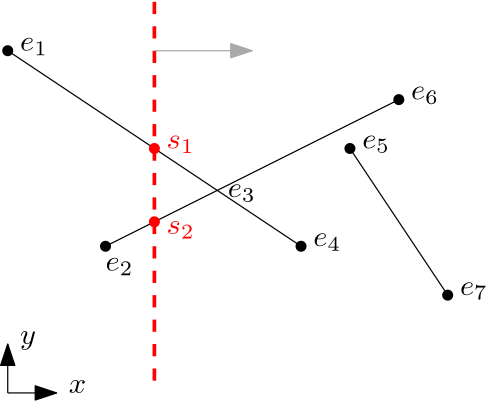
\includegraphics[width=0.6\textwidth]{figs/sweep-line.png}
\شرح{نمایشی از الگوریتمِ جاروبِ خطی برای مسئلهٔ تلاقیِ پاره‌خط‌ها که رخدادها با $e_i$ و داده‌های وضعیت با $s_i$ مشخص شده‌اند.}
\برچسب{شکل:جاروب}
\پایان{شکل}
 
\زیرقسمت{الگوریتم‌های برنامه‌ریزیِ خطی}
طبیعی‌ست که به دلیلِ وجودِ خط‌های راست در مسائلِ هندسی، بسیاری از مسائل به شکلِ برنامه‌ریزی‌های خطی یا برنامه‌ریزی‌های خطیِ تعمیم‌یافته خواهندبود.
برای مثال، هر پاره‌خط نظیرِ یک سه قیدِ خطی‌ست و به سادگی می‌توان متصور شد که مسئلهٔ وجودِ تلاقیِ پاره‌خط‌ها  (تعریف‌شده در \رجوع{مس:برخورد-پاره‌خط}) یا اشیاءِ محدب به سادگی قابلِ تعبیر به مسئلهٔ امکان‌پذیریِ قیودِ برنامه‌ریزیِ خطی باشد. مثالِ دیگری از این دست مسئلهٔ کوچک‌ترین توپِ شامل (تعریف‌شده در \رجوع{مس:توپ-شامل}) است که به شکلِ برنامه‌ریزیِ خطیِ تعمیم‌یافته قابلِ بیان است.
\مرجع{berg}

\زیرقسمت{مسئلهٔ پوشِ محدب}
احتمالاً حذف شود.

\زیرقسمت{مسئلهٔ مثلث‌بندی}
\متن‌سیاه{مسئلهٔ مثلث‌بندی}: یک $N$-ضلعی در صفحه با نقاطِ $p_1$ تا $p_N$ مشخص شده‌اند، مطلوب است لیستی از مثلث‌های $t_1$ تا $t_{N-2}$ به طوری‌که نقطه‌های مثلث‌ها همان نقاطِ چندضلعی باشند و مثلث‌ها بدونِ اشتراک و هم‌پوشانی همهٔ چندضلعی را بپوشانند. 

\شروع{شکل}[آ]
\وسط‌چین

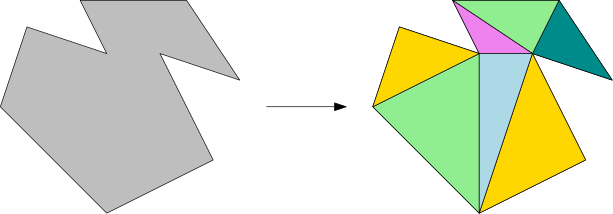
\includegraphics[width=0.6\textwidth]{figs/triangulation.png}
\شرح{یک مثال از مسئلهٔ مثلث‌بندی و پاسخِ آن}
\برچسب{شکل:مثلث‌بندی}
\پایان{شکل}

جوابِ این مسئله یکتا نیست و هرچندضلعی ممکن است به شیوه‌های گوناگونی مثلث‌بندی شود. از این رو مسائلی سخت‌تر از مثلث‌بندی وجود دارند که جوابِ مشخصی دارند، نظیرِ مثلث‌بندی‌ای که مجموعِ طولِ اضلاعِ مثلث‌ها کمینه شود که آن‌را مثلث‌بندیِ کمینه‌وزن می‌نامند. \مرجع{toth} 

 یک الگوریتم برای این مسئله، تقسیمِ چندضلعی به چندضلعی‌های یکنوا و پس از آن مثلث‌بندی‌ست که پیچیدگیِ زمانیِ
$\O{N \log N}$
خواهدداشت.

مسئلهٔ مثلث‌بندی به عنوانِ یک پیش‌پردازشِ کاربردی برای حلِ مسئلهٔ 
وجودِ نقطه در چندضلعی (تعریف شده در \رجوع{مس:نقطه-در-چندضلعی}) یا دیگر مسائلِ برخورد نظیرِ دنبال کردنِ پرتو استفاده می‌شود و از این‌رو اهمیتِ فراوانی در هندسهٔ محاسباتی و گرافیکِ کامپیوتری دارد. \مرجع{berg}

\زیرقسمت{ساختمانِ دادهٔ لیستِ یال‌های دوسویه متصل}

این داده‌ساختار را می‌توان ساده‌ترین و مهم‌ترین داده‌ساختار در ذخیره‌سازیِ اشکالِ هندسی در صفحه دانست. این داده‌ساختار برای افرازهای صفحه استفاده کرد.

این افرازِ صفحه را می‌توان به شکلِ یک گرافِ مسطح دید که برروی آن گره‌ها، یال‌ها و ناحیه‌ها همان نقاط، پاره‌خط‌ها و چندضلعی‌ها هستند که افرازهای صفحه را تشکیل می‌دهند. این گراف غیرجهت‌دار خواهدبود اما می‌توانیم هر یالِ آن را با دو یالِ جهت‌دار که در جهتِ عکسِ یکدیگر قرار گرفته‌اند جایگزین کنیم و به هر یالِ این گرافِ جدید «نیم‌یال» می‌گوییم. دلیلِ این تعریف آن است که آن‌گاه ناحیهٔ چپِ هر نیم‌یال را می‌توانیم به شکلِ دقیقی تعریف کنیم.

این داده‌ساختار متشکل از سه لیست است:
\شروع{شمارش}
    \فقره لیستی از نقاط که برای هر نقطه توابعِ زیر تعریف شده‌اند
    \شروع{شمارش}[-]
        \فقره تابعِ $\mathrm{Coordinates}(v)$ که مختصاتِ نقطهٔ $v$ را بازمی‌گرداند.
        \فقره تابعِ $\mathrm{IncidentEdge}(v)$ که نیم‌یالی دلخواه را بازمی‌گرداند که نقطهٔ شروعش $v$ باشد. 
    \پایان{شمارش}
    \فقره لیستی از نیم‌یال‌ها که برای هر نیم‌یال توابعِ زیر تعریف شده‌اند
    \شروع{شمارش}[-]
        \فقره تابعِ $\mathrm{Origin}(e)$ که نقطهٔ شروعِ نیمی‌یال را مشخص می‌کند.
        \فقره تابعِ $\mathrm{Twin}(e)$ که نیم‌یالی را بازمی‌گرداند که دقیقاً برعکسِ $e$ست.
        \فقره تابعِ $\mathrm{IncidentFace}(e)$ ناحیه‌ای که در چپِ نیم‌یال قرار گرفته‌است را بازمی‌گرداند.
        \فقره تابعِ $\mathrm{Next}(e)$ نیم‌یالی را بازمی‌گرداند که شروعش نقطهٔ پایانِ $e$ باشد و ناحیهٔ سمتِ چپِ این‌دو نیم‌یال با هم یکی باشد.
        \فقره تابعِ $\mathrm{Prev}(e)$ نیم‌یالی را بازمی‌گرداند که پایانش نقطهٔ شروعِ $e$ باشد و ناحیهٔ سمتِ چپِ این‌دو نیم‌یال با هم یکی باشد.
    \پایان{شمارش}
    \فقره لیستی از ناحیه‌ها که برای هر ناحیه توابعِ زیر تعریف شده‌اند
    \شروع{شمارش}[-]
        \فقره تابعِ $\mathrm{OuterComponent}(f)$ اگر ناحیه‌ای وجود دارد که این ناحیه را به طورِ کامل دربر گرفته‌است آن را بازمی‌گرداند.
        \فقره تابعِ $\mathrm{InnerComponents}(v)$ لیستی از ناحیه‌هایی که به طورِ کامل در این ناحیه قرار گرفته‌اند (و با یکدیگر و با ناحیهٔ بیرونی برخورد ندارند) بازمی‌گرداند.
    \پایان{شمارش}
\پایان{شمارش} 

مقادیرِ این توابع محاسبه می‌شوند و در لیست یا دیکشنری نگهداری می‌شوند. با استفاده از این داده‌ساختار می‌توان با آغاز کردن از هر عنصری به همهٔ عناصرِ دیگر دست یافت. \مرجع{berg}

\زیرقسمت{ساختمانِ دادهٔ درختِ کِی‌دی}

\زیرقسمت{دوگانگی}
% Duality
\زیرقسمت{پیش‌پردازش‌های کاربردی، مثالِ دیاگرامِ ورونی}
\برچسب{قس:ورونی}

% TODO

